\documentclass[tikz,border=10pt]{standalone}
\usepackage[utf8]{inputenc}
\usepackage{tikz}
\usetikzlibrary{shapes, arrows.meta, positioning, calc, shadows.blur, backgrounds, fit}

% Definición de colores profesionales (Palette estilo Paper)
\definecolor{paperBlue}{RGB}{70, 130, 180}   % SteelBlue para Audio
\definecolor{paperRed}{RGB}{205, 92, 92}     % IndianRed para Visual
\definecolor{paperGreen}{RGB}{60, 179, 113}  % MediumSeaGreen para Texto
\definecolor{paperOrange}{RGB}{255, 165, 0}  % Orange para Tabular
\definecolor{paperGray}{RGB}{119, 136, 153}  % LightSlateGray para Fusion
\definecolor{loraGold}{RGB}{218, 165, 32}    % GoldenRod para LoRA

\begin{document}

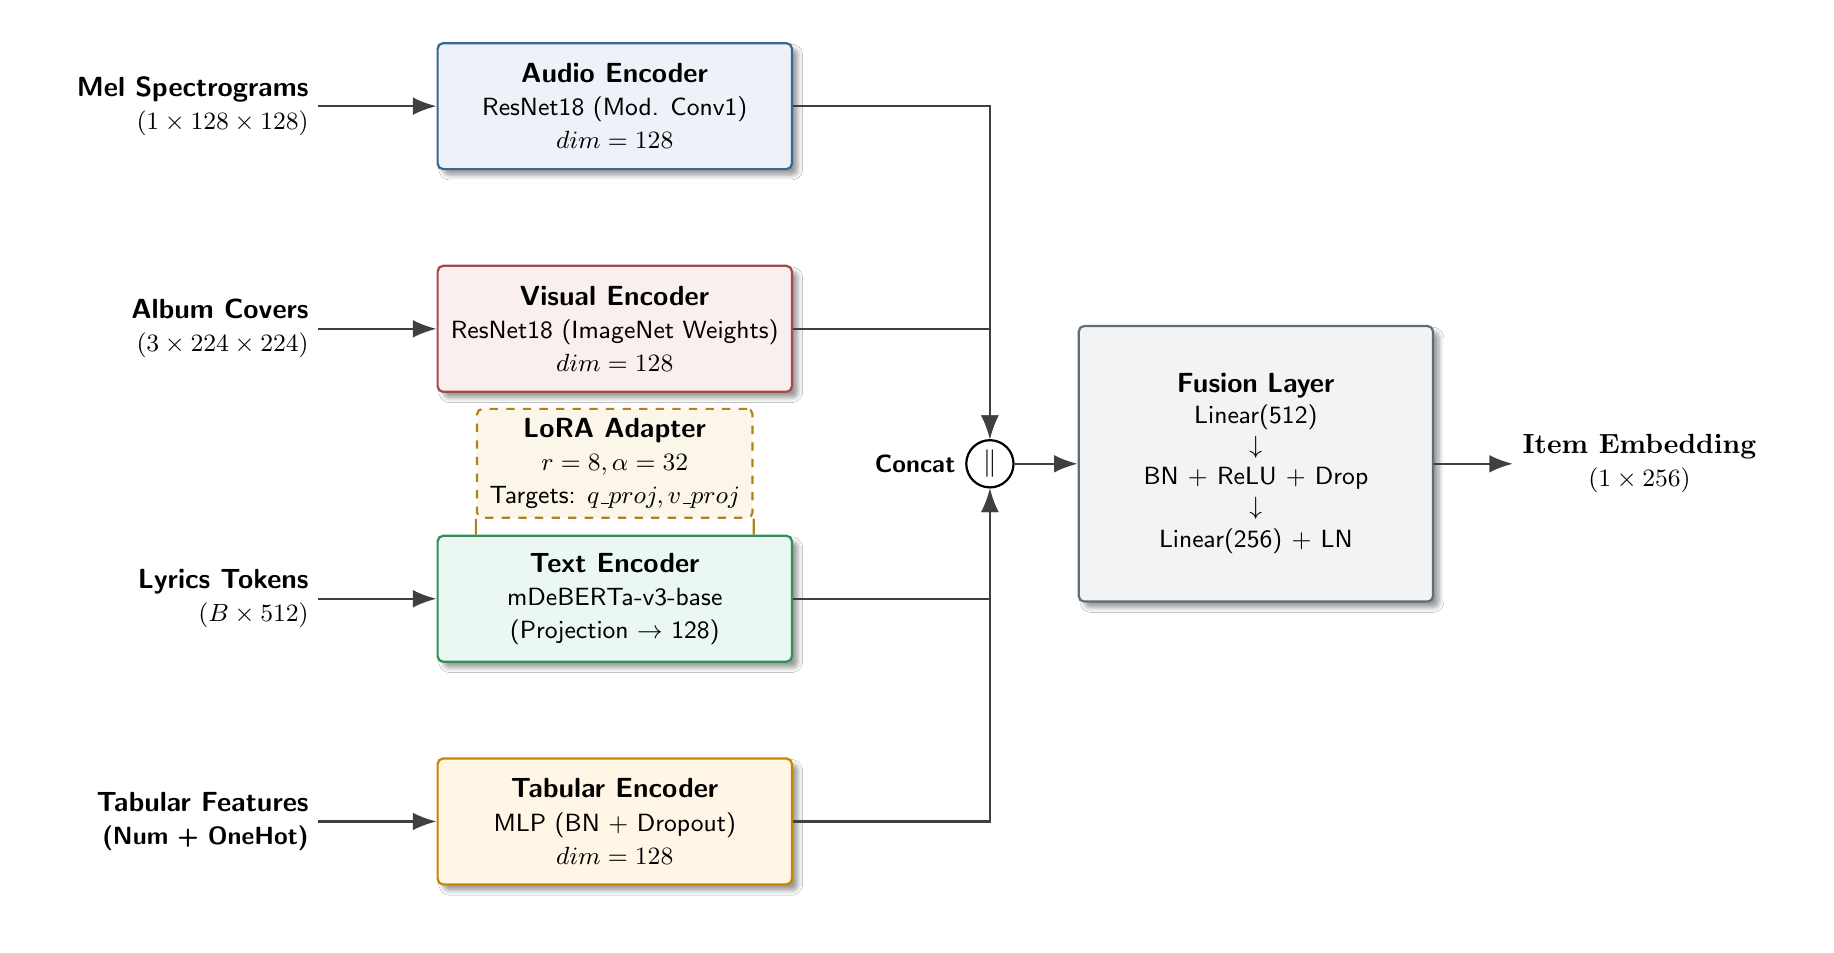
\begin{tikzpicture}[
    node distance=1.2cm and 1.5cm,
    font=\sffamily\normalsize,
    % Estilo base para bloques
    block/.style={
        draw, 
        rounded corners=2pt, 
        minimum height=1.6cm, 
        minimum width=4.5cm, 
        align=center,
        blur shadow={shadow blur steps=5},
        thick
    },
    % Estilo para inputs
    input_node/.style={
        align=right,
        font=\sffamily\bfseries\normalsize
    },
    % Estilo para flechas
    arrow/.style={
        -{Latex[length=3mm]}, 
        thick, 
        darkgray
    },
    % Estilo para el módulo LoRA
    lora/.style={
        draw=loraGold!80!black,
        fill=loraGold!10,
        dashed,
        rounded corners=2pt,
        minimum height=1.2cm,
        minimum width=3.5cm,
        align=center,
        thick
    }
]

    % --- 1. Definición de la Columna de Encoders (Backbones) ---
    
    % Audio Encoder (ResNet18 1-ch)
    \node[block, draw=paperBlue!80!black, fill=paperBlue!10] (audio_enc) {
        \textbf{Audio Encoder}\\
        \small ResNet18 (Mod. Conv1)\\
        \small $dim=128$
    };

    % Visual Encoder (ResNet18 ImageNet) - Debajo de Audio
    \node[block, draw=paperRed!80!black, fill=paperRed!10, below=of audio_enc] (visual_enc) {
        \textbf{Visual Encoder}\\
        \small ResNet18 (ImageNet Weights)\\
        \small $dim=128$
    };

    % Text Encoder (mDeBERTa) - Debajo de Visual
    \node[block, draw=paperGreen!80!black, fill=paperGreen!10, below=1.8cm of visual_enc] (text_enc) {
        \textbf{Text Encoder}\\
        \small mDeBERTa-v3-base\\
        \small (Projection $\rightarrow$ 128)
    };

    % Tabular Encoder (MLP) - Debajo de Texto
    \node[block, draw=paperOrange!80!black, fill=paperOrange!10, below=1.2cm of text_enc] (tab_enc) {
        \textbf{Tabular Encoder}\\
        \small MLP (BN + Dropout)\\
        \small $dim=128$
    };

    % --- 2. Módulo LoRA (Detalle Específico) ---
    % Dibujamos el LoRA "colgando" del Text Encoder como en tu dibujo
    \node[lora, above=0.2cm of text_enc] (lora_mod) {
        \textbf{LoRA Adapter}\\
        \small $r=8, \alpha=32$\\
        \small Targets: $q\_proj, v\_proj$
    };
    
    % Líneas conectando LoRA al backbone principal
    \draw[thick, loraGold!80!black] (text_enc.north west) ++(0.5,0) -- (lora_mod.south west);
    \draw[thick, loraGold!80!black] (text_enc.north east) ++(-0.5,0) -- (lora_mod.south east);

    % --- 3. Inputs (Izquierda) ---
    
    % Input Audio
    \node[input_node, left=1.5cm of audio_enc] (in_audio) {
        Mel Spectrograms\\
        \small $(1 \times 128 \times 128)$
    };
    \draw[arrow] (in_audio) -- (audio_enc);

    % Input Visual
    \node[input_node, left=1.5cm of visual_enc] (in_img) {
        Album Covers\\
        \small $(3 \times 224 \times 224)$
    };
    \draw[arrow] (in_img) -- (visual_enc);

    % Input Text
    \node[input_node, left=1.5cm of text_enc] (in_text) {
        Lyrics Tokens\\
        \small $(B \times 512)$
    };
    \draw[arrow] (in_text) -- (text_enc);

    % Input Tabular
    \node[input_node, left=1.5cm of tab_enc] (in_tab) {
        Tabular Features\\
        \small (Num + OneHot)
    };
    \draw[arrow] (in_tab) -- (tab_enc);

    % --- 4. Fusion Layer (Derecha) ---
    
    % Nodo de Concatenación (simbólico)
    \coordinate (concat_point) at ($(visual_enc.east)!0.5!(text_enc.east) + (2.5, 0)$);
    
    \node[circle, draw, thick, fill=white, inner sep=1pt, minimum size=0.6cm, label={180:\sffamily\bfseries\small Concat}] (concat) at (concat_point) {$\parallel$};
    
    % Flechas hacia la concatenación
    \draw[arrow] (audio_enc.east) -| (concat);
    \draw[arrow] (visual_enc.east) -- (concat_point |- visual_enc.east) -- (concat);
    \draw[arrow] (text_enc.east) -- (concat_point |- text_enc.east) -- (concat);
    \draw[arrow] (tab_enc.east) -| (concat);

    % Bloque de Fusión Final
    \node[block, draw=paperGray!80!black, fill=paperGray!10, right=0.8cm of concat, minimum height=3.5cm, text width=3.5cm] (fusion_layer) {
        \textbf{Fusion Layer}\\
        \small Linear(512)\\
        $\downarrow$\\
        \small BN + ReLU + Drop\\
        $\downarrow$\\
        \small Linear(256) + LN
    };

    \draw[arrow] (concat) -- (fusion_layer);

    % --- 5. Output Final ---
    \node[right=1cm of fusion_layer, font=\bfseries, align=center] (final_out) {Item Embedding\\ \small $(1 \times 256)$};
    \draw[arrow] (fusion_layer) -- (final_out);

    % --- Fondo y Labels Generales (Opcional) ---
    \begin{scope}[on background layer]
        \node[fit=(in_audio)(tab_enc)(final_out), fill=white, inner sep=0.5cm] {};
    \end{scope}

\end{tikzpicture}
\end{document}